\documentclass[12pt]{article}
\usepackage{graphicx}
\usepackage{amsmath}
\usepackage{geometry}
\usepackage{listings}
\usepackage{float}
\usepackage{booktabs}  
\usepackage{array}
\geometry{margin=1in}

\title{CS 3502 - Project 1 \\ Multi-Threaded Banking System}
\author{Tanner Giddens}
\date{\today}

\begin{document}
\maketitle

\section{Introduction}
This project demonstrates core multi-threading concepts in C using POSIX threads:
race conditions, mutual exclusion (mutexes), deadlock, and deadlock prevention.
The work is divided into four phases that progressively show the problem and the fix.

\section{Implementation Overview}

\subsection{Phase 1: Race Condition}
Phase 1 runs multiple teller threads that perform deposits and withdrawals on shared
account balances without synchronization. Because updates are not protected,
read-modify-write sequences interleave and corrupt shared state. The program prints
the expected total versus the actual total and reports when a race condition is detected.

\subsection{Phase 2: Mutex Protection}
Phase 2 adds per-account mutex locks to protect critical sections during transfers.
Transfers acquire both required account locks (with lock ordering) before modifying balances,
ensuring totals remain consistent. This phase also measures and prints execution time.

\subsection{Phase 3: Deadlock Demonstration}
Phase 3 intentionally creates deadlock by acquiring two account locks in inconsistent order
across two threads (0$\rightarrow$1 and 1$\rightarrow$0). This satisfies the Coffman conditions:
mutual exclusion, hold and wait, no preemption, and circular wait. The program detects
stalled progress and reports suspected deadlock after a timeout.

\subsection{Phase 4: Deadlock Prevention}
Phase 4 prevents deadlock using consistent lock ordering. All transfers acquire locks in the
same global order (lowest account ID first), eliminating circular wait. The program completes
successfully, preserves the total balance, and prints execution time.

\section{Screenshots}
All screenshots are taken from terminal output runs on Ubuntu (VMware Workstation).

\subsection{Phase 1 Output}
\begin{figure}[H]
\centering
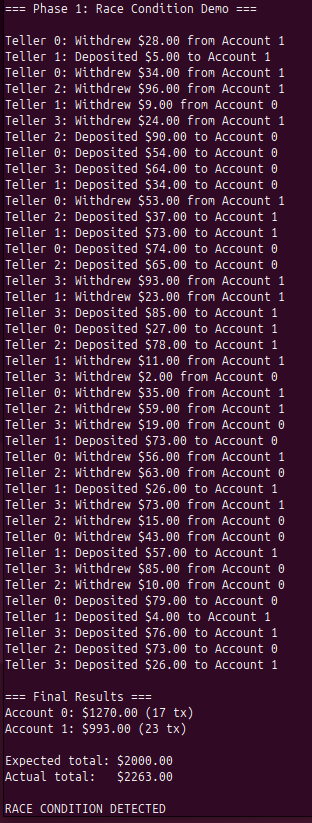
\includegraphics[width=0.9\linewidth,height=0.75\textheight,keepaspectratio]{Phase1.png}
\caption{Phase 1: Race condition detected (expected vs actual totals differ).}
\end{figure}

\subsection{Phase 2 Output}
\begin{figure}[H]
\centering
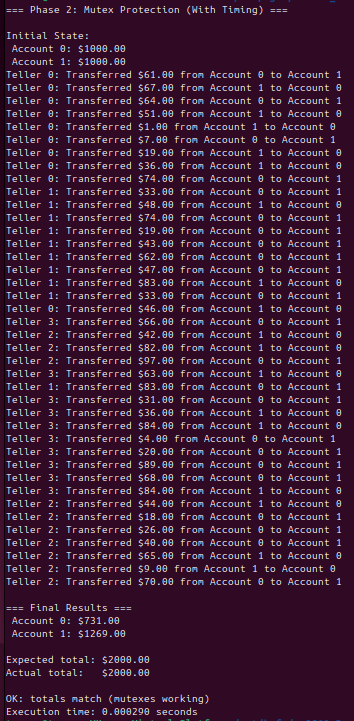
\includegraphics[width=0.9\linewidth,height=0.75\textheight,keepaspectratio]{Phase2.png}
\caption{Phase 2: Mutex protection preserves totals and prints execution time.}
\end{figure}

\subsection{Phase 3 Output}
\begin{figure}[H]
\centering
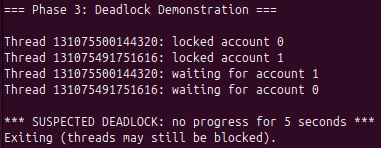
\includegraphics[width=0.95\textwidth]{Phase3.png}
\caption{Phase 3: Deadlock scenario with both threads waiting; timeout detects stalled progress.}
\end{figure}

\subsection{Phase 4 Output}
\begin{figure}[H]
\centering
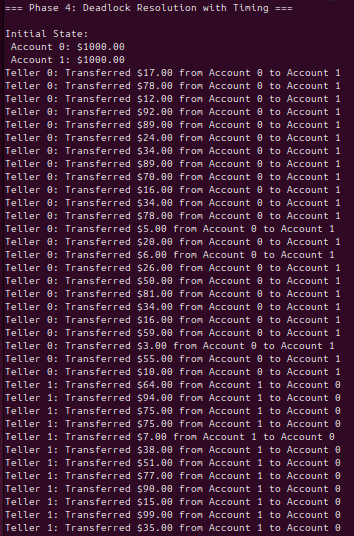
\includegraphics[width=0.95\textwidth]{Phase4 part1.png}
\caption{Phase 4 (Part 1): Transfer output while running with lock ordering.}
\end{figure}

\begin{figure}[H]
\centering
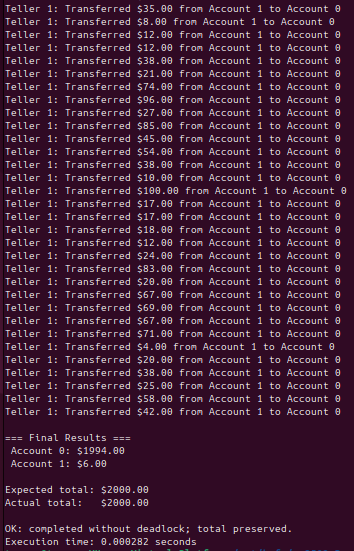
\includegraphics[width=0.95\textwidth]{Phase4 part2.png}
\caption{Phase 4 (Part 2): Final results showing total preserved and execution time.}
\end{figure}

\section{Performance Analysis}

\subsection{Timing Results}
Execution time is measured using clock\_gettime(CLOCK\_MONOTONIC, ...).
Table~\ref{tab:timings} summarizes timing results from multiple runs.

\begin{table}[H]
\centering
\caption{Execution time (seconds) across runs.}
\label{tab:timings}
\begin{tabular}{@{}lcccc@{}}
\toprule
Phase & Run 1 & Run 2 & Run 3 & Average \\ \midrule
Phase 2 (mutex) & 0.000293 & 0.000335 & 0.000365 & 0.000331 \\
Phase 4 (ordered locks) & 0.000879 & 0.000381 & 0.000210 & 0.000490 \\
\bottomrule
\end{tabular}
\end{table}

\subsection{Discussion}

Phase 1 may appear faster because it does not use synchronization, but it produces
incorrect and inconsistent results due to race conditions. As shown in Table~\ref{tab:timings},
both Phase 2 and Phase 4 introduce slight locking overhead to ensure correctness.
Although Phase 4 includes additional lock ordering logic to prevent circular wait,
its execution time remains comparable to Phase 2. The measured differences are on the
order of microseconds and are negligible relative to the benefit of guaranteed
correctness and deadlock prevention. Phase 4 consistently completed without
deadlock, even when threads performed opposing transfers.

\subsection{Challenges and Solutions}
\begin{enumerate}

\item \textbf{Challenge 1: Identifying the Race Condition} \\
\textbf{Answer:} In Phase 1, the race condition was difficult to identify at first because the program did not
 always produce incorrect results. Sometimes the final balance appeared correct, which made the issue seem
 inconsistent. After running the program multiple times and comparing totals, I realized that the shared balance
 variable was being modified without synchronization during the read, modify, write sequence.

\item \textbf{Challenge 2: Debugging Deadlock} \\
\textbf{Answer:} In Phase 3, the program would occasionally freeze without printing additional output. It was not
 immediately clear whether the program had crashed or was stuck waiting indefinitely. By adding print statements
 around the lock acquisition calls, I observed that two threads were each holding one lock while waiting for the
 other, confirming that a circular wait condition had formed.

\item \textbf{Challenge 3: Designing a Deadlock-Free Solution} \\
\textbf{Answer:} Implementing lock ordering in Phase 4 required restructuring the transfer logic carefully. I
 needed to ensure that correctness was preserved while preventing circular wait. By enforcing a consistent global
 ordering rule where threads always lock the lower-index account first, I was able to eliminate deadlock while
 maintaining correct transfers.

\item \textbf{Challenge 4: Measuring Performance Accurately} \\
\textbf{Answer:} Because the program executes in microseconds, performance differences between phases were small
 and difficult to observe. To obtain more reliable results, I used clock\_gettime(CLOCK\_MONOTONIC, ...)
 for high-resolution timing and averaged multiple runs to reduce variability.
\end{enumerate}

\section{Reflection Questions (16)}

\begin{enumerate}
\item \textbf{Reflection 1.1: Race Condition Evidence} \\
\textbf{Answer:} When I ran Phase 1 five times, I did not get the same final balance each time. The totals frequently differed
 from the expected \$2000.00 because multiple threads were modifying shared balances without synchronization. The race condition occurs
 in the deposit and withdrawal functions where the balance is read, modified, and written back without a mutex. The specific issue
 happens during the read, modify, write sequence where one thread reads the balance while another thread updates it at the same time.

\item \textbf{Reflection 1.2: Thread vs Process} \\
\textbf{Answer:} A process is an independent program with its own separate address space, while a thread is a lightweight
 execution unit that runs inside a process. Threads within the same process share memory, including global variables and heap memory,
 which allows faster communication. Processes do not share memory by default, which provides isolation and protection. Threads share
 memory because they exist within the same process context and use the same address space. 

\item \textbf{Reflection 1.3: pthread\_join Purpose} \\
\textbf{Answer:} When I removed the pthread\_join() calls, the program often ended before the worker threads finished executing.
 This caused incomplete output and inconsistent results. pthread\_join() is necessary because it forces the main thread to wait until all
 created threads have completed. Without it, the main thread may exit early and terminate the entire process.

\item \textbf{Reflection 1.4: Non-Determinism} \\
\textbf{Answer:} Non-deterministic behavior means that a program can produce different results even when run multiple times with the
 same input. In concurrent programs, the operating system scheduler determines the order in which threads execute, and this order can change
 each run. This makes debugging difficult because errors may appear randomly and cannot always be reproduced easily. Race conditions
 especially depend on timing, which is unpredictable.

\item \textbf{Reflection 2.1: Correctness Variation} \\
\textbf{Answer:} When I ran Phase 2 ten times, the final balances were always correct. The total consistently remained \$2000.00
 across all runs. This differs from Phase 1, where the totals changed due to race conditions. The use of mutex locks ensures that only one
 thread modifies shared data at a time, preserving correctness.

\item \textbf{Reflection 2.2: Critical Solutions} \\
\textbf{Answer:} A critical section is a portion of code where shared data is accessed and must not be executed by more than one
 thread simultaneously. In Phase 2, the critical sections occur inside the transfer function where account balances are modified. The code
 between pthread\_mutex\_lock() and pthread\_mutex\_unlock() protects these shared updates. This ensures atomic transfer operations.

\item \textbf{Reflection 2.3: Performance Trade-offs} \\
\textbf{Answer:} Phase 1 executes slightly faster because it does not use locks, but it produces incorrect results. Phase 2 is
 slightly slower due to the overhead of acquiring and releasing mutexes. This slowdown is acceptable because correctness is more important
 than speed in financial systems. Ensuring data integrity outweighs minor performance costs.

\item \textbf{Reflection 2.4: Granularity} \\
\textbf{Answer:} Each account has its own mutex to allow greater parallelism. With per-account locks, threads can operate on
 different accounts at the same time without blocking each other. If a single global mutex were used, only one transfer could occur at a
 time, reducing concurrency. Fine-grained locking improves performance while maintaining correctness.

\item \textbf{Reflection 3.1: Coffman Conditions} \\
\textbf{Answer:} Mutual exclusion exists because each account lock allows only one thread at a time. Hold and wait occurs when a
 thread locks one account and waits for the second lock. No preemption is present because a lock cannot be forcibly removed from a thread.
 Circular wait happens when Thread A waits for a lock held by Thread B, while Thread B waits for a lock held by Thread A.

\item \textbf{Reflection 3.2: Resource Allocation Graph} \\
\textbf{Answer:} In the deadlock scenario, each thread holds one account lock and waits for the other. Thread 1 holds Account 0
 and waits for Account 1, while Thread 2 holds Account 1 and waits for Account 0. This creates a circular dependency between the threads
 and resources. The cycle in the graph visually demonstrates why deadlock occurs.

\item \textbf{Reflection 3.3: Deadlock vs Livelock} \\
\textbf{Answer:} Deadlock occurs when threads are permanently blocked waiting for resources held by each other. Livelock occurs when
 threads continue running but repeatedly retry operations without making progress. My program experiences deadlock, not livelock, because both
 threads become completely blocked and stop executing. There is no active retry behavior.

\item \textbf{Reflection 3.4: Real-World Example} \\
\textbf{Answer:} One real-world example of deadlock occurred in database management systems such as Microsoft SQL Server, where
 transactions could lock tables in inconsistent order. This sometimes caused database transactions to freeze until the system detected and
 resolved the deadlock. Database deadlocks can interrupt service and impact reliability in production systems. This shows why proper lock
 management is critical in real-world applications.

\textbf{Source:} Microsoft Learn. ``Deadlocks in SQL Server.''
https://learn.microsoft.com/en-us/sql/relational-databases/sql-server-deadlocks-guide

\item \textbf{Reflection 4.1: Breaking Circular Wait} \\
\textbf{Answer:} Lock ordering prevents deadlock by eliminating circular wait. Since all threads acquire locks in the same global
 order, it is impossible to form a cycle of dependencies. By removing circular wait, one of the four Coffman conditions is no longer satisfied.
 Without all four conditions, deadlock cannot occur.

\item \textbf{Reflection 4.2: Strategy Comparison} \\
\textbf{Answer:} Deadlock detection allows flexibility but requires monitoring and possible recovery actions. Deadlock prevention through
 lock ordering avoids the issue entirely by design. Detection may be useful in complex systems where ordering is not practical. In this project,
 prevention is simpler and more efficient.

\item \textbf{Reflection 4.3: Starvation} \\
\textbf{Answer:} Lock ordering can potentially cause starvation if one thread repeatedly acquires locks before another thread is scheduled.
 However, in this implementation the critical sections are short, so starvation is unlikely. With fair scheduling by the operating system, threads
 generally get equal opportunities to execute. Therefore, starvation risk is minimal here.

\item \textbf{Reflection 4.4: Production Recommendation} \\
\textbf{Answer:} For a real banking system, I would recommend deadlock prevention using lock ordering. Prevention is better than detection
 because it avoids system freezes entirely. Financial systems require strong consistency and availability, so avoiding deadlock is critical. Lock
 ordering provides a simple and reliable strategy for ensuring safe concurrent transactions.
\end{enumerate}

\section{Conclusion}
This project showed how unsynchronized shared memory updates cause race conditions,
how mutexes enforce safe critical sections, how deadlock can be created through inconsistent
lock acquisition, and how deadlock can be prevented using lock ordering. The final phases
maintained correctness and completed reliably while measuring performance.

\end{document}
